\chapter{Two fission modes in $^{178}$Pt}\label{chap:178Pt}

\section{Asymmetric fission in the region of $^{180}$Hg}
As mentioned in the introduction, fission has been studied most carefully in the region of the actinides (Z=90 to Z=103), since naturally-occurring isotopes in this region are fissile. Within this region, there is a characteristic tendency for fission fragment yields to be asymmetric (that is, one light fragment and one heavy fragment), with the heavy peak centered around $A\approx140$~\cite{unik1974}. This has been understood as a manifestation of nuclear shell structure in the prefragments: doubly-magic $^{132}$Sn drives the nucleus towards scission, and once the neck nucleons are divided up between the two fragments, the heavy fragment distribution peaks near A=140~\cite{Wilkins1976}. As one moves to the lighter nuclei, however, this tendency becomes less and less pronounced as yields tend to become more symmetric~\cite{Schmidt2000,Schmidt2001}. For sub-thorium isotopes, there is no doubly-magic nucleus candidate that could drive the system toward asymmetry as there is with actinides. To the contrary: neutron-deficient {\Hg}, for instance, might be expected to split evenly into two $^{90}$Zr fragments, each with $N=50$ closed neutron shells.

However, it was reported in a 2010 study~\cite{Andreyev2010} that neutron-deficient $^{180}$Tl undergoes beta-delayed fission, leading to the excited intermediate state {\Hg} which in turn decays into two fragments of unequal mass. This finding triggered a flurry of theoretical papers trying to explain this new and unexpected phenomenon (for instance, see~\cite{Warda2012,Moller2012,Mcdonnell2014,Ichikawa2019}). Meanwhile, a follow-up study using $^{178}$Tl~\cite{Liberati2013} further established that this was a region of asymmetric fission, and not just a one-time occurrence. Since then, other nuclei in the region have been studied using a variety of reactions and techniques, each with mass asymmetric fragments. An overview of fission fragment distributions in the region of {\Hg} which have been experimentally studied (as of 2016), marked by the experimental technique used, is shown in Figure~\ref{fig:178ptregion}.

%Nuclei in this region have a number of unique features which make them interesting for study, even aside from the unexpected fragment asymmetry. Predicted fission barrier heights in this region are relatively-low (of the order of ~12 MeV), making them suitable for study using low-energy techniques such as $\beta$-delayed fission (maybe~\cite{Andreyev2013} and the work at ISOLDE at CERN?) or Coulex-induced fission (maybe~\cite{Martin2015} and the SOFIA (Studies On FIssion with Aladin) experiment/project/campaign). On the other hand, it has been found that compound nuclei formed in this region from particle-induced reactions tend to have high excitation energies, even for beam energies near the Coulomb barrier. This combination makes the region particularly well-suited for studies involving a variety of excitation energies.

%Furthermore, later experiments have shown that, unlike the case of actinides where shell structure and fragment asymmetry are ``washed out'' at high excitation energies, mass asymmetric fragment distributions are a persistent feature of this mass region for various excitation energies (see~\cite{Andreyev2018} and references therein). An overview of fission fragment ditributions in the region of {\Hg} which have been experimentally studied (as of 2016), marked by the experimental technique used, is shown in Figure~\ref{fig:178ptregion}.

\begin{figure}
	\centering
	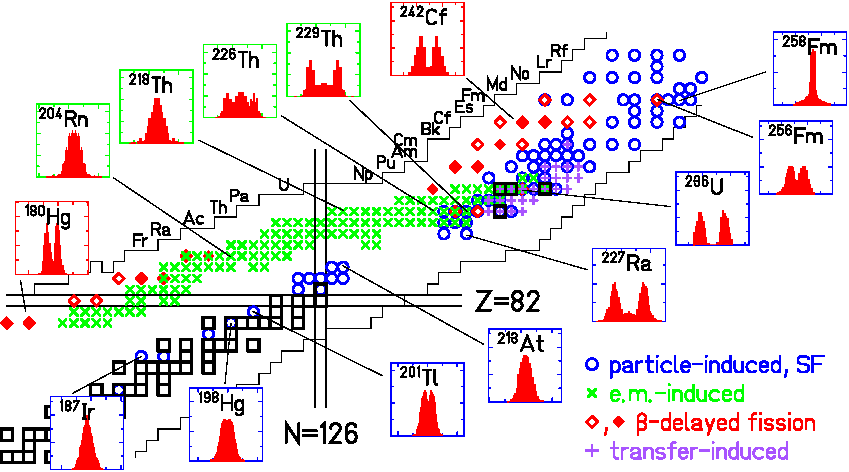
\includegraphics[width=0.9\linewidth]{./TeX_files/178Pt_region}
	\caption[Fragment yields as a function of $N$ and $Z$ for several nuclei ranging from actinides, where primary fission yields tend to be asymmetric, down to near-thorium, where yields become more symmetric, and finally to the region near neutron deficient {\Hg}, where asymmetry returns.]{Fragment yields as a function of $N$ and $Z$ for several nuclei ranging from actinides, where primary fission yields tend to be asymmetric, down to near-thorium, where yields become more symmetric, and finally to the region near neutron deficient {\Hg}, where asymmetry returns. Figure from~\cite{Andreyev2018}.}
	\label{fig:178ptregion}
\end{figure}



\section{Multimodal fission of $^{178}$Pt}\label{sect:178Ptfrags}

One particular follow-up experiment was performed to investigate the fission of {\Pt}~\cite{Tsekhanovich2019}, which differs from {\Hg} by 2 protons. This system was studied at various excitation energies and found to fission consistently in a bimodal pattern, as shown in Figure~\ref{fig:178ptexptdata}. Of the sample measured, roughly 1/3 of cases were found to fission symmetrically, while the other 2/3 fissioned asymmetrically with a light-to-heavy mass ratio of approximately 79/99. Furthermore, it was observed that mass-asymmetric fragments tended to have higher kinetic energies than symmetric fragments.

\begin{figure}
	\centering
	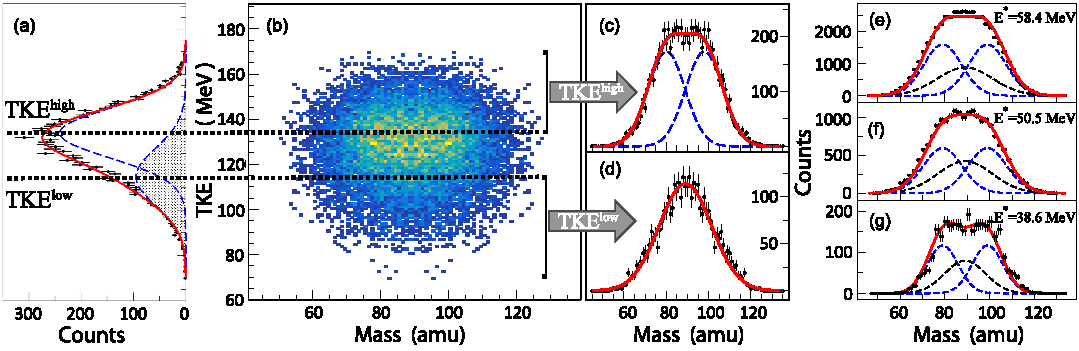
\includegraphics[width=0.95\linewidth]{TeX_files/178Pt_expt_data}
	\caption[After projecting the fission fragment mass vs total kinetic energy (TKE) correlation (b) onto the TKE axis, the TKE distribution is deconvoluted into high- and low-energy components, centered around the values TKE$^\mathrm{high}$ and TKE$^\mathrm{low}$ (a). The mass distributions at these particular energies are fitted to a double (c) and single (d) Gaussian, respectively. This procedure is repeated for three different compound nucleus excitation energies E* (e-g).]{After projecting the fission fragment mass vs total kinetic energy (TKE) correlation (b) onto the TKE axis, the TKE distribution is deconvoluted into high- and low-energy components, centered around the values TKE$^\mathrm{high}$ and TKE$^\mathrm{low}$ (a). The mass distributions at these particular energies are fitted to a double (c) and single (d) Gaussian, respectively. This procedure is repeated for three different compound nucleus excitation energies E* (e-g). Figure from~\cite{Tsekhanovich2019}.}
	\label{fig:178ptexptdata}
\end{figure}

To better interpret the results of this experiment, we performed DFT calculations using the Skyrme functional {\hfb}~\cite{Schunck2015} and the Gogny functional D1S~\cite{Berger1989}. These calculations involved computing a PES using the collective coordinates $Q_{20}$ and $Q_{30}$. The {\hfb} PES is shown in Figure~\ref{fig:178ptunedf1pes}, and the D1S PES is in Figure~\ref{fig:178ptd1spes}. A calculation with full Langevin dynamics was not performed because the framework was still being developed at the time; however, the static (minimum-energy) pathways shown in the figures correspond to a fragment split $A_L/A_H \approx 80/98$, in good agreement with the experimental ratio $A_L/A_H \approx 79/99$.

\begin{figure}
	\centering
	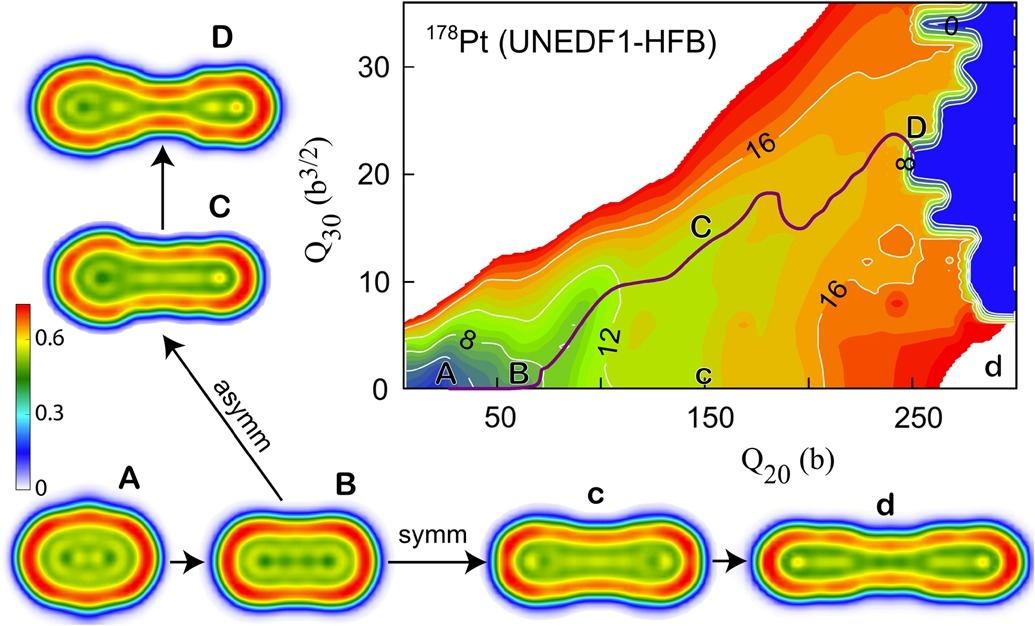
\includegraphics[width=0.7\linewidth]{TeX_files/178Pt_unedf1_pes.jpg}
	\caption[UNEDF1$_\mathrm{HFB}$ potential energy surface for $^{178}$Pt as a function of multipole moments $Q_{20}$, representing elongation, and $Q_{30}$, representing mass asymmetry. The static pathway is marked in purple. Note the two different trajectories ABCD and ABcd and their corresponding NLFs.]{UNEDF1$_\mathrm{HFB}$ potential energy surface for $^{178}$Pt as a function of multipole moments $Q_{20}$, representing elongation, and $Q_{30}$, representing mass asymmetry. The static pathway is marked in purple. Note the two different trajectories ABCD and ABcd and their corresponding NLFs.}
	\label{fig:178ptunedf1pes}
\end{figure}

Also shown in Figure~\ref{fig:178ptunedf1pes} are nucleon localization functions (recall Section~\ref{sect:locali}) corresponding to various marked configurations in the PES. Along the symmetric path (ABcd in the figure), the fragments appear highly-elongated, including shortly before scission. Since elongation tends to minimize the Coulomb repulsion between fragments, then this configuration might be expected to lead to fragments with relatively low kinetic energies. On the other hand, compact fragments such as those in ABCD will tend to have a larger Coulomb repulsion, resulting in compact asymmetric fragments with a higher kinetic energy, which is in qualitative agreement with experiment.

Comparing the {\hfb} PES in Figure~\ref{fig:178ptunedf1pes} to the D1S PES in Figure~\ref{fig:178ptd1spes}a, one may note that, despite the inherent differences between the functionals, the overall topography of the PES is similar in both cases. In fact, the topography in both cases is quite flat, which suggests (in agreement with the observed data) the possibility of a competition between symmetric and asymmetric fission modes. Additionally, as shown in Figure~\ref{fig:178ptd1spes}b, there appears an additional channel corresponding to compact symmetric fragments. This channel is higher in energy than the elongated symmetric pathway and is blocked by a ${\sim}4$ MeV saddle point, but it is conceivable that this channel might be more easily accessed at higher $E^*$. %This possibility is being explored for potential future experiments [cite: private conversations with Igor]

\begin{figure}
	\centering
	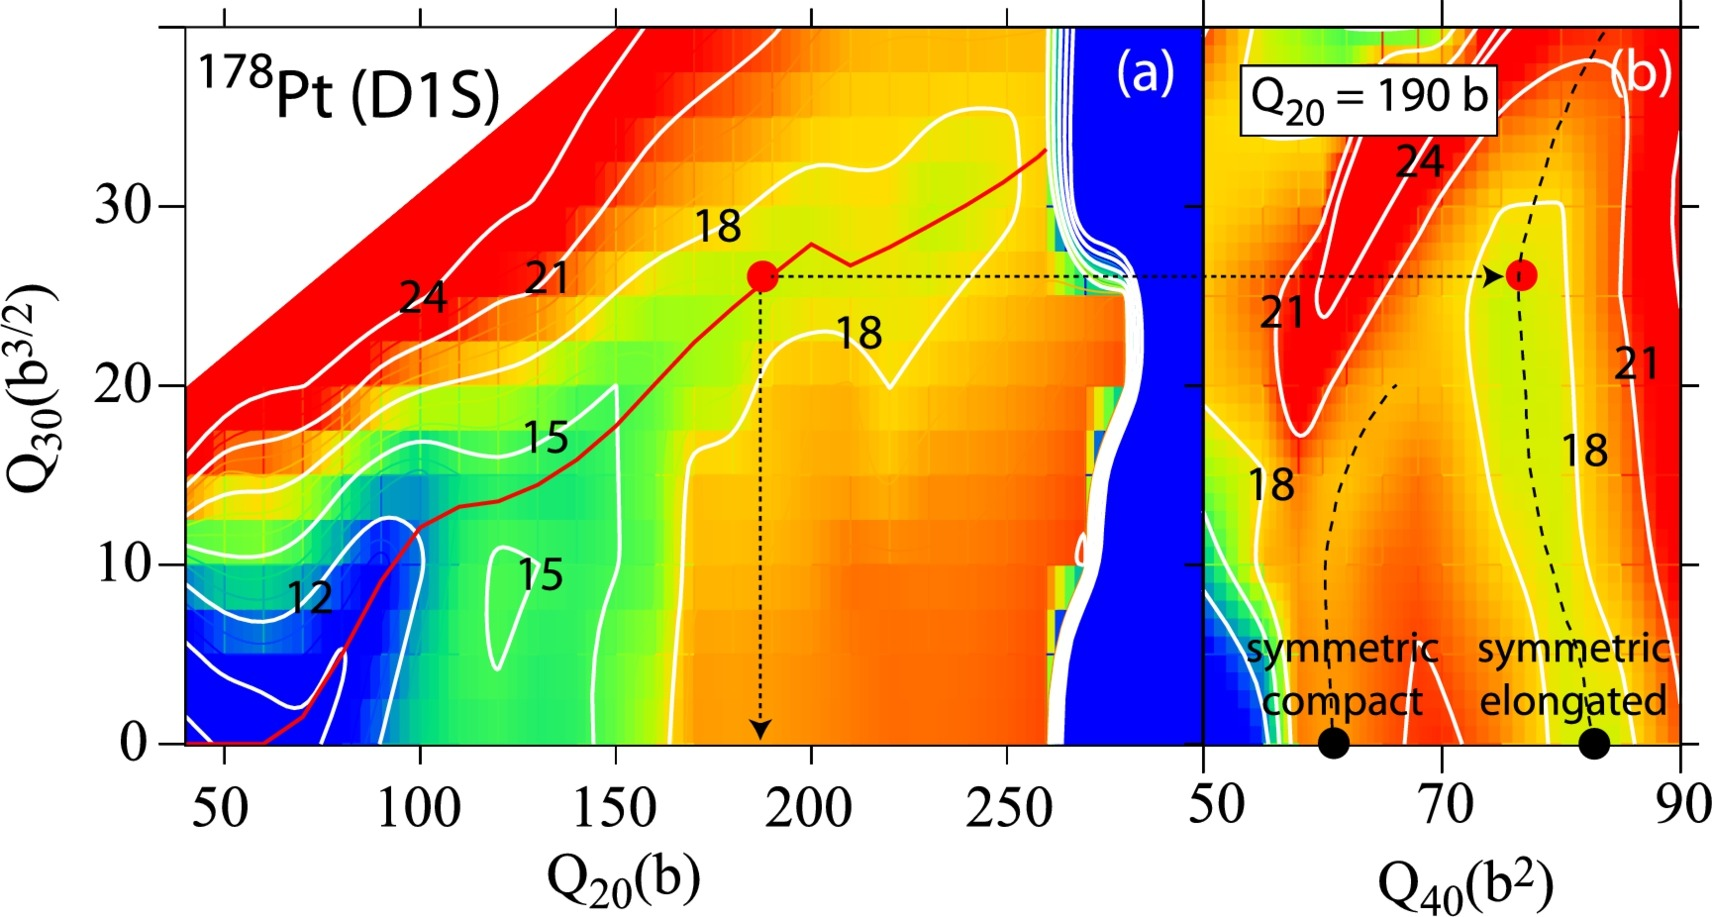
\includegraphics[width=0.7\linewidth]{TeX_files/178Pt_D1S_pes.jpg}
	\caption[a) D1S potential energy surface for $^{178}$Pt as a function of multipole moments $Q_{20}$, representing elongation, and $Q_{30}$, representing mass asymmetry. The static pathway is marked in red. b) With the quadrupole moment fixed to $Q_{20}=190$b, a PES is constructed as a function of $Q_{40}$, which relates to the size of the neck, and $Q_{30}$. This PES shows the existence of two symmetric modes, separated by a saddle point with a height of ${\sim}4$ MeV.]{a) D1S potential energy surface for $^{178}$Pt as a function of multipole moments $Q_{20}$, representing elongation, and $Q_{30}$, representing mass asymmetry. The static pathway is marked in red. b) With the quadrupole moment fixed to $Q_{20}=190$b, a PES is constructed as a function of $Q_{40}$, which relates to the size of the neck, and $Q_{30}$. This PES shows the existence of two symmetric modes, separated by a saddle point with a height of ${\sim}4$ MeV.}
	\label{fig:178ptd1spes}
\end{figure}



\section{The physical origin of fragment asymmetry in the neutron-deficient sub-lead region}

By now it is now well-established that many isotopes in the neutron-deficient sub-lead region will fission asymmetrically. Microscopic-macroscopic calculations correctly predict asymmetry in the yields, and static DFT calculations do even better by predicting the peak of the distribution to within 1-2 nucleons. In that sense, it may be said that the phenomenon is understood. That said, a simple, intuitive interpretation or explanation of that phenomenon is still a matter of some debate.

After the discovery of asymmetric fission in {\Hg}, one of the earliest theoretical responses~\cite{Moller2012} argued that no simple explanation or intuitive interpretation is possible, and that the best explanation for the observation, however unsatisfying, is simply the sum total of all the physics that gets wrapped together to compute a PES. Fragment yields are determined by subtle interplays in local regions of the potential energy surface, while magic number-based arguments are just a lot of fortuitous hand-waving that happens to work well for actinides. The fact of asymmetric fragments, in this explanation, is something that happens in spite of, and not because of, fragment shell effects (which, two of the authors later note~\cite{Ichikawa2012}, are rather weak in this region).

By contrast, it is argued in~\cite{Warda2012a} that the fragment masses are determined by the shell structure of two well-formed prefragments connected by a thin neck. The nucleons in the neck are then redistributed to either of the prefragments somewhere along the way from saddle point to scission. This argument was further reinforced in a follow-up paper~\cite{Mcdonnell2014}, in which it is shown that the asymmetric path is associated with stronger shell effects than the symmetric path.

Two more recent papers~\cite{Scamps2018a, scamps2019} fundamentally agree with this second perspective, except they argue that one should consider the shell structure of octupole-deformed prefragments instead of familiar spherical magic numbers. By their reasoning, octupole softness would favor fragment distributions with $Z_{light}\approx34$ and $N_{heavy}\approx56$.

Most recently, an argument is presented in~\cite{Ichikawa2019} which likewise invokes deformed shell gaps; however, in this case the argument is made for octupole-deformed (or rather, mass asymmetric) parent nuclei, as opposed to octupole-deformed fragments.

Taken together, these suggest that fragment asymmetry is the result of a coupling between highly-deformed shell gaps in the parent nucleus and (possibly-deformed) shell gaps in the fragment nuclei. The separation process might also introduce some additional complications, which may involve dissipation and particle emission.

So far, no microscopic dynamical description has been given for fission in this region. It would be interesting to see how the collective inertia behaves for these nuclides, and how they affect the fission dynamics.

